


\begin{exercise}
\label{exerc:08-02-periodicsequence}
Consider the pair of confocal conics ($\E_1$, $\E_2$, $\Hc_1$ and $\Hc_2$) as shown in  \cref{fig:retangulo_exerc82}.

  Consider a ray starting at $F_1$ intersecting the branch $\Hc_2$ at $P_1$ and  the ray
  $F_2P_1$  intersecting the ellipse $\E_2$  at $P_2$. Analogously, we define the points $P_3=P_2F_1\cap\Hc_1$, $P_4=P_3F_2\cap\E_1$, $P_5=P_4F_1\cap\Hc_2$,
  $P_6$, etc.  
  
\noindent i) Determine conditions to obtain $P_5=P_1$. 
In this case show that the perimeter of the quadrilateral
$P_1P_2P_3P_4$ is constant, i.e., independent of the position of the point $P_1$.  See \cite{dolgirev2014}.


\noindent ii) Analyze the cases when $P_1=\E_2\cap \Hc_2$ or $P_1=\E_1\cap \Hc_2$.

 \begin{figure}[H]
 	\begin{center}
 	 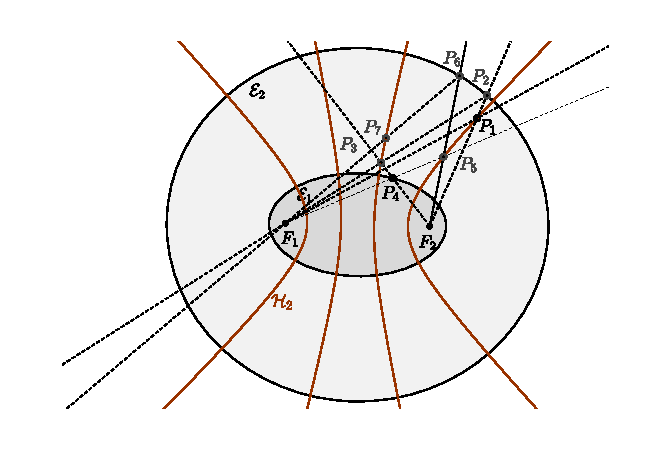
\includegraphics[scale=1]{chap_09/pics/pics_09_910_dinamica_retangulos.pdf}
 		\caption {Sequence of points $P_1,  \,P_2, \ldots,  P_5 ,  \ldots$  
 		 \label{fig:retangulo_exerc82} }
 	\end{center}
 	\end{figure}
 	
 	\end{exercise}